\section{How JSP Works}
\begin{figure}[htbp]
\begin{center}
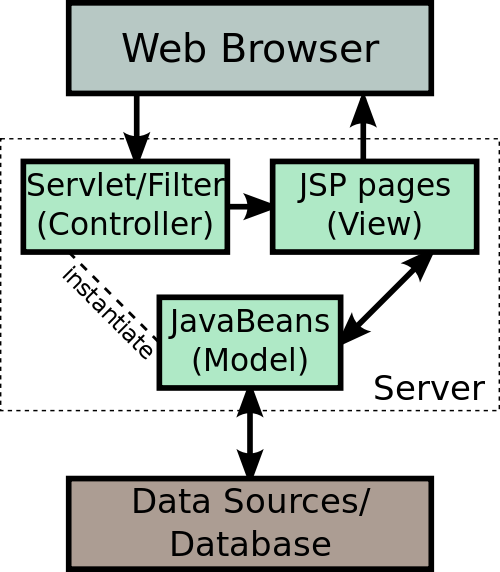
\includegraphics[width=6cm]{./NetworkingTechnologies/jsp/JSP.png}
\caption{Architecture of Java Server Pages}
\label{jsp}
\end{center}
\end{figure}



A JSP page exist in 3 forms.
\begin{enumerate}
	\item \textbf{JSP source code}   This is the version the developer actually writes. it consist of a text file with \texttt{.jsp} extension, and contains a mix of HTML template code, Java language statements, and JSP directives and actions that describe how to generate a Web page to service a particular request.
	\item \textbf{Java Source Code}   The JSP container translates the JSP source code into the source code for an equivalent Java servlet as needed. This source code os typically saved in a work area and is often helpful for debugging.
	\item \textbf{Compiled Java class}   Like any other Java class, the generated servlet code is compiled into byte codes in a \texttt{.class} file, ready to be loaded and executed.
\end{enumerate}
The JSP container manages each of these forms of JSP page automatically, based on the timestamp of each file. In response to an HTTP request, the container checks to see if the \texttt{.jsp} source has been modified since the \texttt{.java} source was last compiled. If so, the container retranslates the JSP source code into Java source and recompiles it. When a request for JSP page is made, the container first determines the name of the class corresponding to \texttt{.jsp} file. If class doesn't exits or is older than \texttt{.jsp} file, then the container creates java source code for equivalent servlet and recompiles it. Then the container loads the servlet class and creates an instance. Finally the container dispatches a thread to handle the current HTTP request in loaded instance.